\documentclass[tikz,10pt,fleqn]{article}

\setlength{\parskip}{0.5\baselineskip}%
\usepackage[utf8]{inputenc}
% a4paper
\usepackage[a4paper, margin={1in,1in}]{geometry}
\usepackage[titletoc,title]{appendix}
\usepackage{latexsym}
\usepackage{amssymb}
\usepackage{gensymb}
\usepackage{amsmath}
\usepackage{amsfonts}
\usepackage[dvipsnames]{xcolor}
\usepackage{multicol}
\usepackage{graphicx}
\usepackage{fancyhdr}
\usepackage[linguistics]{forest}
\usepackage{colortbl}
\usepackage{pdfpages}
\usepackage{wrapfig}
\usepackage{cancel}
\usepackage{multirow}
\usepackage[export]{adjustbox}
\usepackage{tabularx}
\newcolumntype{C}{>{\centering\arraybackslash}X }

% \makeatletter
% \newcommand{\currentfontsize}{\fontsize{\f@size}{\f@baselineskip}\selectfont}
% \makeatother

\usepackage{minted}
\definecolor{LightGray}{gray}{0.95}
\setminted{
    frame=lines,
    framesep=2mm,
    baselinestretch=1.2,
    bgcolor=LightGray,
    fontsize=\fontsize{8.5}{8.5}\selectfont,
    linenos,
    mathescape=true,
    % escapeinside=||,
}
% \setmintedinline{
%     fontsize=\fontsize{8.5}{8.5}\selectfont,
% }

\definecolor{darkblue}{rgb}{0.0, 0.0, 1}
\usepackage[pdftex,hyperfigures,hyperindex,bookmarksnumbered,colorlinks, bookmarks, breaklinks, linktocpage,citecolor=darkblue,urlcolor=darkblue,linkcolor=darkblue,pagebackref=true,linktoc=all]{hyperref}
\usepackage{cleveref}

% to fixme
\usepackage{xcolor} 
\definecolor{FIXMECOLOR}{rgb}{1,0,0}
\newcommand{\FIXME}[1]{{\color{FIXMECOLOR}{\textbf{FIXME: #1}}}} 

% to simplify math 

\newcommand{\bvec}[1]{
   \ensuremath{
   \begin{bmatrix}
       #1 \\
   \end{bmatrix}
}}

\newcommand{\bmat}[1]{
   \ensuremath{
   \begin{bmatrix}
       #1
   \end{bmatrix}
}}

\newcommand{\dotprod}[2]{\ensuremath{\left< #1, #2 \right>}}

%% For plotting
\usepackage{pgfplots}
\pgfplotsset{width=10cm,compat=1.9}
\usepgfplotslibrary{external}
\tikzexternalize
%%
\usepackage{dirtree}
\usepackage{subcaption}
\usepackage{xifthen}% provides \isempty test
\usepackage{glossaries}

\captionsetup[subfigure]{labelformat=empty}
\definecolor{color1}{HTML}{0B0C10}
\definecolor{color2}{HTML}{1F2833}
\definecolor{color3}{HTML}{C5C6C7}
\definecolor{color4}{HTML}{66FCF1}
\definecolor{color5}{HTML}{45A29E}

\pagestyle{fancy}
\fancyhf{}
%%%%%%%%%%%%%%%%%%%%%%%%%%%%
%% VARIABLES
\newcommand\namesurname{Alessandro Gobbetti}
\newcommand\assignment{Project: Make it Stand}

\newcommand\subject{Computational Fabrication}
% today's date
\newcommand\documentdate{\today}

% Title content
%%%%%%%%%%%%%%%%%%%%%%%%%%%%
\rhead{\assignment}
\lhead{\namesurname}
%%%%%%%%%%%%%%%%%%%%%%%%%%%%
\rfoot{Page \thepage}
\setlength{\parindent}{0pt}

\newcommand\xdownarrow[1][2ex]{%
   \mathrel{\rotatebox{90}{$\xleftarrow{\rule{#1}{0pt}}$}}
}

\begin{document}

\begin{titlepage}
    \begin{center}
        \vspace*{2cm}

        \textbf{\Large{\assignment}}

        \vspace{0.5cm}
        \textbf{\subject}\\[5mm]
        % \assignment


        % \vspace{1.8cm}

        \namesurname
        \vspace{1.8cm}

        { \hypersetup{hidelinks} \tableofcontents }
        \vspace*{\fill}

        
\includegraphics[width=0.4\textwidth]{fig/logo}

        \documentdate \\
        Università della Svizzera italiana\\
        Faculty of Informatics\\
        Switzerland\\

    \end{center}
\end{titlepage}

% \newpage
% { \hypersetup{hidelinks} \tableofcontents }
% \newpage
% In this assignment you will be testing capabilities of one of our 3D printers (Ultimaker S5). To this end, you
% will first design a testing pattern/geometry, similar to those above, using constructive solid geometry tool
% (OpenSCAD). Then, you will print and investigate the resulting quality. Finally, you will create a short report
% describing the capabilities of the printer.

\section{Introduction}
This project aims at stabilizing shapes for 3D fabrication. The main idea is to carve the interior of the object to move the center of mass in a way that the object can stand on its own. The project is inspired by the work of \cite{Pevost:2013:MIS}.

\section{Method}
An object is considered stable if its center of mass lies on top of the convex support polygon.

\subsection{Volume Representation}
To simplify the problem, the mesh is first voxelized. This is done by creating a grid of voxels and checking if the center of the voxel is inside the mesh by shooting rays in multiple directions and counting the number of intersections with the mesh. If the number of intersections is odd, the voxel is considered inside the mesh. The ray directions are chosen following the Fibonacci sphere algorithm to ensure a uniform distribution of rays and then applying some random jittering to avoid artifacts.

Since every voxel computation is independent, the algorithm can be parallelized using OpenMP to speed up the voxelization process.

\subsection{Identifying the Convex Support Polygon}
The base of the object is the set of voxels in the lowest layer of the object.
The object is balanced not only if the barycenter lies in the base but also if the barycenter lies on top of the convex hull of the base. The convex hull is computed using the Graham scan algorithm. A starting point is chosen as the point with the lowest $y$ coordinate, and the points are sorted by the angle they form with the starting point. The first two points always belong to the convex hull, for the rest of the points, we keep track of the last three points in the convex hull and check if the new point forms a left turn with the last two points. If it does not, we remove the last point from the convex hull until the new point forms a left turn with the last two points. The algorithm is $O(n \log n)$, where $n$ is the number of points.

\begin{figure}[h]
    \centering
    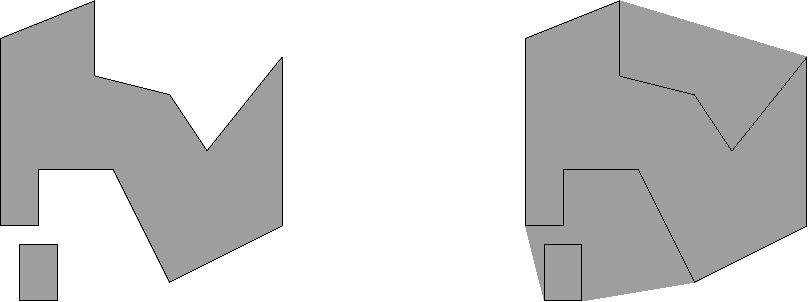
\includegraphics[width=0.5\textwidth]{fig/convex_hull.pdf}
    \caption{Convex hull of a complex shape: left the original shape, right the convex polygon.}
    \label{fig:convex_hull}
\end{figure}

The polygon is then triangulated to keep a voxelized representation of the convex hull for future easier computation of the barycenter.

\subsection{Center of Mass}
The center of mass is computed as the sum of the mass of each voxel times its position divided by the total mass. In this case, we consider 1 as the mass of each voxel that is inside the object and 0 otherwise. The center of mass is then projected on the convex hull to check if it lies inside. If it does not, the object is not stable.

\subsection{Stabilizing the Object}
To stabilize the object, we need to move the center of mass on top of the convex hull. This can be done by carving the object (removing voxels from the interior of the object). But which voxels should be removed? We first determine the direction from the barycenter to the closest point on the convex hull. We then define two semiplanes orthogonal to this direction that intersect at the barycenter (see \autoref{fig:semiplane}). If any voxel on top of the semiplane not containing the convex hull is removed, the center of mass will move towards the convex hull, thus improving the stability of the object.

\begin{figure}[h]
    \centering
    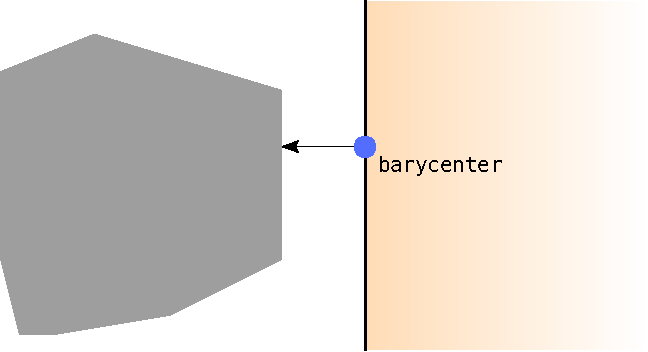
\includegraphics[width=0.5\textwidth]{fig/semiplane.pdf}
    \caption{The barycenter (in blue) and the semiplane (in orange) defined by the direction from the barycenter to the closest point on the convex hull.}
    \label{fig:semiplane}
\end{figure}

Due to voxelization, and in cases where the barycenter is already close to the convex hull, the direction might not be accurate. To improve the accuracy, we consider the closest 16 voxels in the base to the barycenter and we average them to get a more accurate direction.

The interior voxels of the object are then sorted by the distance from the semiplane. The voxels are removed starting from the farthest ones (that have a higher impact on the center of mass) until the center of mass lies on top of the convex hull. 

The interior voxels are previously marked as such by checking their distance from the exterior voxels. For further stability, the convex hull can also be eroded to avoid the barycenter being on the edge of it making the object more stable.

During the carving process, the semiplanes are recalculated every $n$ voxels removed to ensure the direction is still accurate.

\section{Expanding the Base}
Contrary to the paper~\cite{Pevost:2013:MIS}, the shape of the object is not deformed, instead when stability is not achieved with carving, the base is dilated in the direction of the barycenter. The base is expanded by adding voxels in the direction of the barycenter until the center of mass lies on top of the convex hull or a maximum number of iterations is reached. For fabrication purposes, voxels are not added only in the layer of the base but also in the layers above it to ensure the object is stable.

\section{Results}
To test the performance of the algorithm, we created inclined rectangular prisms with different angles: 10\degree, 15\degree and 20\degree. The results are shown in \autoref{fig:prisms}.
The prism (a) was already stable without any carving. The prism (b) was carved to achieve stability. The prims (c) at 20\degree was not stabilized by carving, but its base was expanded to make it stand on its own as shown in (d). In this way, the object is not deformed, and the original shape is preserved and a small number of voxels are added to the base to stabilize the object.

\begin{figure}[H]
    {
    \centering
    
\includegraphics[width=0.8\textwidth]{fig/carved.png}\\
    }
    
    \hspace{1.9cm} (a) \hspace{2.4cm} (b) \hspace{2.4cm} (c) \hspace{2.9cm} (d)

    \caption{Inclined rectangular prisms with different angles: (a) 10\degree, (b) 15\degree, (c) and (d) 20\degree. The light gray voxels are the exterior voxels, the dark gray voxels are the interior voxels. The base of (d) has been expanded to stabilize the object.}
    \label{fig:prisms}
\end{figure}

A more complex shape is shown in \autoref{fig:complex}. The banana shape was stabilized by carving the interior of the object. The base was also dilated in the direction of the barycenter to further stabilize the object.
\begin{figure}[H]
    \centering
    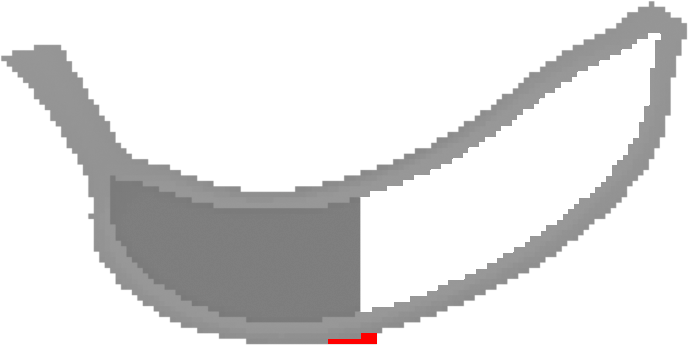
\includegraphics[width=0.6\textwidth]{fig/banana_carved.png}
    \caption{Complex shape of a banana. The light gray voxels are the exterior voxels, the dark gray voxels are the interior voxels. In white the removed voxels. The base has been expanded (in red) to further stabilize the object.}
    \label{fig:complex}
\end{figure}

Another example is the model of the monster-like figure shown in \autoref{fig:monster}. The object was inclined and balanced on its head and the base was slightly expanded to stabilize it.

\begin{figure}[H]
    \centering
    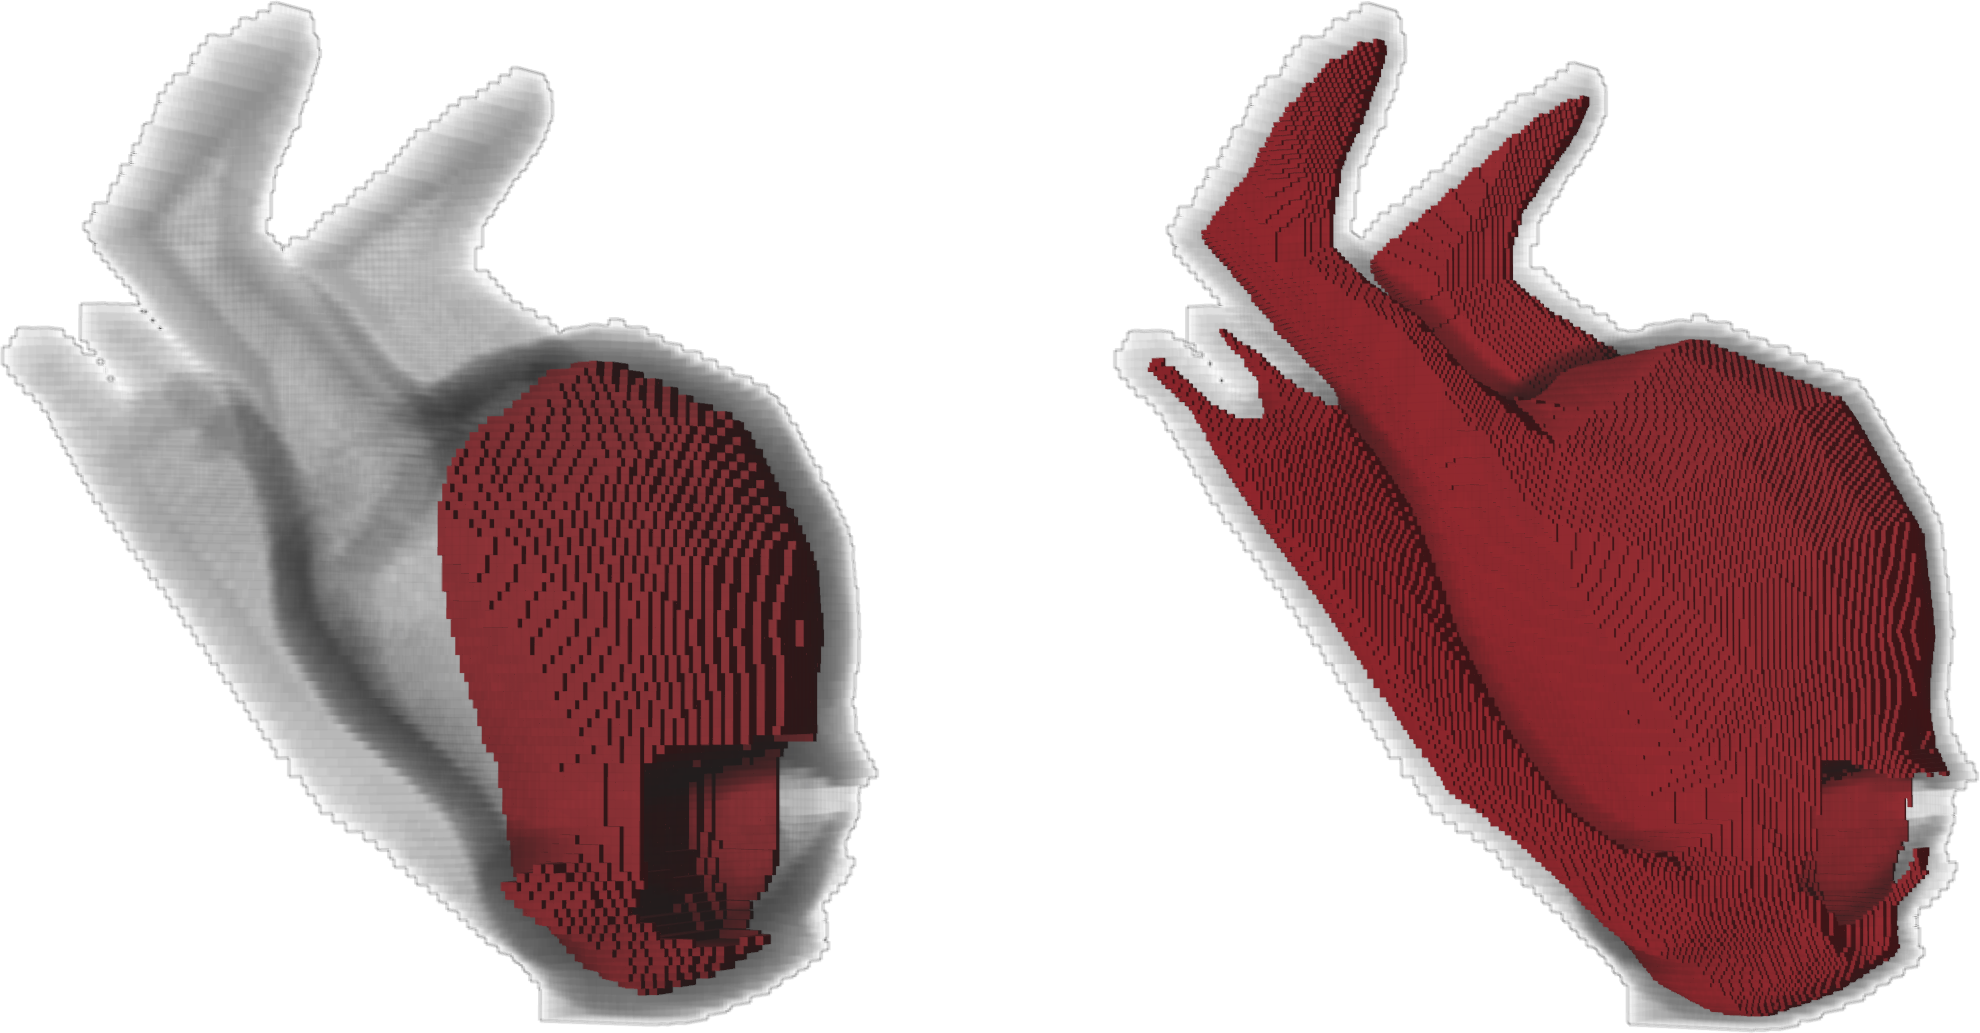
\includegraphics[width=0.7\textwidth]{fig/mrhumpty.png}
    \caption{Monster-like figure. In red the interior voxels, in gray the rest of the voxels. The base has been expanded to stabilize the object. Left: stabilized object, right: original object.}
    \label{fig:monster}
\end{figure}


\section{Running the Code}
The code is written in C++ and uses cmake to compile. It has been successfully tested on Linux and MacOS. To compile the code, run the following commands:
\begin{minted}{bash}
mkdir build
cd build
cmake ..
make
\end{minted}

To run the code, navigate to the \mintinline{bash}{build} directory and run the following command:
\begin{minted}{bash}
./make_it_stand <input_file> <output_file> [OPTIONS]
\end{minted}
where \mintinline{bash}{<input_file>} and \mintinline{bash}{<output_file>} are obj files and the options are:
\begin{itemize}
    \item \mintinline{bash}{--dim <dimension>}: Dimension of voxel grid (default: 32)
    \item \mintinline{bash}{--num-rays <number>}: Number of rays per voxel (default: 2)
    \item \mintinline{bash}{--jitter <jitter>}: Jittering factor for ray directions (default: 0.1)
    \item \mintinline{bash}{--distance <distance>}: Distance to mesh surface when carving (default: 3)
    \item \mintinline{bash}{--base-distance <distance>}: Distance to base border when computing stability (default: 1)
    \item \mintinline{bash}{--max-base-dilation <number>}: Number of iterations for base expansion (default: 10)
    \item \mintinline{bash}{--help}: Display help message
\end{itemize}   





\bibliographystyle{plain}
\bibliography{bibliography}
\end{document}





